\documentclass{extbook}[14pt]
\usepackage{multicol, enumerate, enumitem, hyperref, color, soul, setspace, parskip, fancyhdr, amssymb, amsthm, amsmath, latexsym, units, mathtools}
\everymath{\displaystyle}
\usepackage[headsep=0.5cm,headheight=0cm, left=1 in,right= 1 in,top= 1 in,bottom= 1 in]{geometry}
\usepackage{dashrule}  % Package to use the command below to create lines between items
\newcommand{\litem}[1]{\item #1

\rule{\textwidth}{0.4pt}}
\pagestyle{fancy}
\lhead{}
\chead{Answer Key for Progress Quiz 7 Version A}
\rhead{}
\lfoot{4173-5738}
\cfoot{}
\rfoot{Spring 2021}
\begin{document}
\textbf{This key should allow you to understand why you choose the option you did (beyond just getting a question right or wrong). \href{https://xronos.clas.ufl.edu/mac1105spring2020/courseDescriptionAndMisc/Exams/LearningFromResults}{More instructions on how to use this key can be found here}.}

\textbf{If you have a suggestion to make the keys better, \href{https://forms.gle/CZkbZmPbC9XALEE88}{please fill out the short survey here}.}

\textit{Note: This key is auto-generated and may contain issues and/or errors. The keys are reviewed after each exam to ensure grading is done accurately. If there are issues (like duplicate options), they are noted in the offline gradebook. The keys are a work-in-progress to give students as many resources to improve as possible.}

\rule{\textwidth}{0.4pt}

\begin{enumerate}\litem{
Construct the lowest-degree polynomial given the zeros below. Then, choose the intervals that contain the coefficients of the polynomial in the form $ax^3+bx^2+cx+d$.
\[ -7, \frac{7}{2}, \text{ and } \frac{1}{2} \]The solution is \( 4x^{3} +12 x^{2} -105 x + 49 \), which is option D.\begin{enumerate}[label=\Alph*.]
\item \( a \in [-3, 6], b \in [-47, -42], c \in [117, 124], \text{ and } d \in [-51, -39] \)

$4x^{3} -44 x^{2} +119 x -49$, which corresponds to multiplying out $(x -7)(2x -7)(2x -1)$.
\item \( a \in [-3, 6], b \in [-18, -15], c \in [-100, -89], \text{ and } d \in [48, 54] \)

$4x^{3} -16 x^{2} -91 x + 49$, which corresponds to multiplying out $(x -7)(2x + 7)(2x -1)$.
\item \( a \in [-3, 6], b \in [-15, -8], c \in [-109, -101], \text{ and } d \in [-51, -39] \)

$4x^{3} -12 x^{2} -105 x -49$, which corresponds to multiplying out $(x -7)(2x + 7)(2x + 1)$.
\item \( a \in [-3, 6], b \in [12, 17], c \in [-109, -101], \text{ and } d \in [48, 54] \)

* $4x^{3} +12 x^{2} -105 x + 49$, which is the correct option.
\item \( a \in [-3, 6], b \in [12, 17], c \in [-109, -101], \text{ and } d \in [-51, -39] \)

$4x^{3} +12 x^{2} -105 x -49$, which corresponds to multiplying everything correctly except the constant term.
\end{enumerate}

\textbf{General Comment:} To construct the lowest-degree polynomial, you want to multiply out $(x + 7)(2x -7)(2x -1)$
}
\litem{
Which of the following equations \textit{could} be of the graph presented below?

\begin{center}
    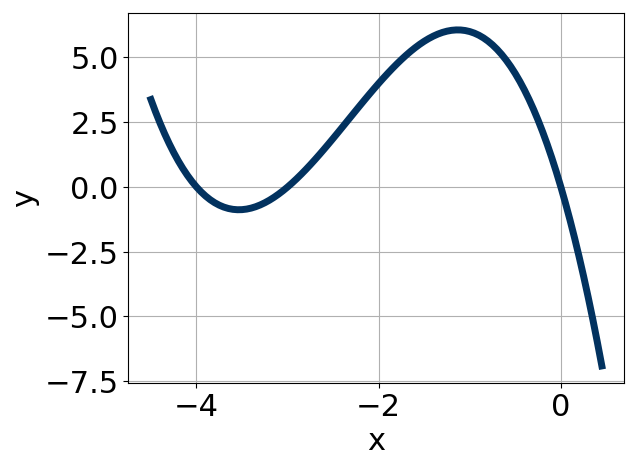
\includegraphics[width=0.5\textwidth]{../Figures/polyGraphToFunctionA.png}
\end{center}


The solution is \( 13x^{7} (x - 1)^{7} (x - 3)^{11} \), which is option A.\begin{enumerate}[label=\Alph*.]
\item \( 13x^{7} (x - 1)^{7} (x - 3)^{11} \)

* This is the correct option.
\item \( -18x^{9} (x - 1)^{10} (x - 3)^{9} \)

The factor $(x - 1)$ should have an odd power and the leading coefficient should be the opposite sign.
\item \( -15x^{5} (x - 1)^{11} (x - 3)^{11} \)

This corresponds to the leading coefficient being the opposite value than it should be.
\item \( 8x^{9} (x - 1)^{8} (x - 3)^{5} \)

The factor $1$ should have been an odd power.
\item \( 3x^{7} (x - 1)^{4} (x - 3)^{10} \)

The factors $1$ and $3$ have have been odd power.
\end{enumerate}

\textbf{General Comment:} General Comments: Draw the x-axis to determine which zeros are touching (and so have even multiplicity) or cross (and have odd multiplicity).
}
\litem{
Describe the zero behavior of the zero $x = -9$ of the polynomial below.
\[ f(x) = 8(x - 9)^{5}(x + 9)^{8}(x - 8)^{6}(x + 8)^{8} \]The solution is the graph below, which is option B.
\begin{center}
    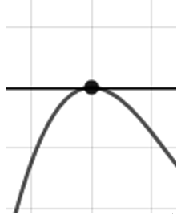
\includegraphics[width=0.3\textwidth]{../Figures/polyZeroBehaviorBA.png}
\end{center}\begin{enumerate}[label=\Alph*.]
\begin{multicols}{2}
\item 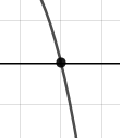
\includegraphics[width = 0.3\textwidth]{../Figures/polyZeroBehaviorAA.png}
\item 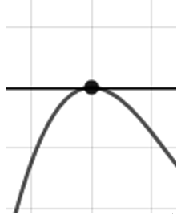
\includegraphics[width = 0.3\textwidth]{../Figures/polyZeroBehaviorBA.png}
\item 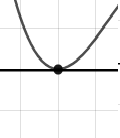
\includegraphics[width = 0.3\textwidth]{../Figures/polyZeroBehaviorCA.png}
\item 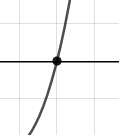
\includegraphics[width = 0.3\textwidth]{../Figures/polyZeroBehaviorDA.png}
\end{multicols}\item None of the above.\end{enumerate}
\textbf{General Comment:} You will need to sketch the entire graph, then zoom in on the zero the question asks about.
}
\litem{
Construct the lowest-degree polynomial given the zeros below. Then, choose the intervals that contain the coefficients of the polynomial in the form $x^3+bx^2+cx+d$.
\[ -2 - 3 i \text{ and } -3 \]The solution is \( x^{3} +7 x^{2} +25 x + 39 \), which is option D.\begin{enumerate}[label=\Alph*.]
\item \( b \in [1, 4], c \in [5.44, 8.1], \text{ and } d \in [8.6, 9.7] \)

$x^{3} + x^{2} +6 x + 9$, which corresponds to multiplying out $(x + 3)(x + 3)$.
\item \( b \in [-13, -5], c \in [23.8, 26.58], \text{ and } d \in [-41.4, -37.8] \)

$x^{3} -7 x^{2} +25 x -39$, which corresponds to multiplying out $(x-(-2 - 3 i))(x-(-2 + 3 i))(x -3)$.
\item \( b \in [1, 4], c \in [3.4, 5.01], \text{ and } d \in [5.2, 6.9] \)

$x^{3} + x^{2} +5 x + 6$, which corresponds to multiplying out $(x + 2)(x + 3)$.
\item \( b \in [2, 15], c \in [23.8, 26.58], \text{ and } d \in [37.2, 41.1] \)

* $x^{3} +7 x^{2} +25 x + 39$, which is the correct option.
\item \( \text{None of the above.} \)

This corresponds to making an unanticipated error or not understanding how to use nonreal complex numbers to create the lowest-degree polynomial. If you chose this and are not sure what you did wrong, please contact the coordinator for help.
\end{enumerate}

\textbf{General Comment:} Remember that the conjugate of $a+bi$ is $a-bi$. Since these zeros always come in pairs, we need to multiply out $(x-(-2 - 3 i))(x-(-2 + 3 i))(x-(-3))$.
}
\litem{
Construct the lowest-degree polynomial given the zeros below. Then, choose the intervals that contain the coefficients of the polynomial in the form $ax^3+bx^2+cx+d$.
\[ -5, -2, \text{ and } 3 \]The solution is \( x^{3} +4 x^{2} -11 x -30 \), which is option E.\begin{enumerate}[label=\Alph*.]
\item \( a \in [-5, 6], b \in [-4.3, -3.7], c \in [-13, -6], \text{ and } d \in [25, 37] \)

$x^{3} -4 x^{2} -11 x + 30$, which corresponds to multiplying out $(x -5)(x -2)(x + 3)$.
\item \( a \in [-5, 6], b \in [1.6, 4.9], c \in [-13, -6], \text{ and } d \in [25, 37] \)

$x^{3} +4 x^{2} -11 x + 30$, which corresponds to multiplying everything correctly except the constant term.
\item \( a \in [-5, 6], b \in [-6.1, -5.4], c \in [-9, 1], \text{ and } d \in [25, 37] \)

$x^{3} -6 x^{2} -x + 30$, which corresponds to multiplying out $(x -5)(x + 2)(x -3)$.
\item \( a \in [-5, 6], b \in [-10.9, -9.5], c \in [29, 36], \text{ and } d \in [-30, -23] \)

$x^{3} -10 x^{2} +31 x -30$, which corresponds to multiplying out $(x -5)(x -2)(x -3)$.
\item \( a \in [-5, 6], b \in [1.6, 4.9], c \in [-13, -6], \text{ and } d \in [-30, -23] \)

* $x^{3} +4 x^{2} -11 x -30$, which is the correct option.
\end{enumerate}

\textbf{General Comment:} To construct the lowest-degree polynomial, you want to multiply out $(x + 5)(x + 2)(x -3)$
}
\litem{
Describe the zero behavior of the zero $x = 4$ of the polynomial below.
\[ f(x) = 8(x - 4)^{5}(x + 4)^{8}(x - 8)^{3}(x + 8)^{5} \]The solution is the graph below, which is option A.
\begin{center}
    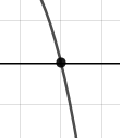
\includegraphics[width=0.3\textwidth]{../Figures/polyZeroBehaviorCopyAA.png}
\end{center}\begin{enumerate}[label=\Alph*.]
\begin{multicols}{2}
\item 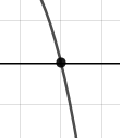
\includegraphics[width = 0.3\textwidth]{../Figures/polyZeroBehaviorCopyAA.png}
\item 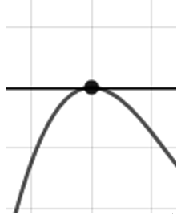
\includegraphics[width = 0.3\textwidth]{../Figures/polyZeroBehaviorCopyBA.png}
\item 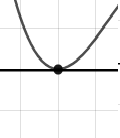
\includegraphics[width = 0.3\textwidth]{../Figures/polyZeroBehaviorCopyCA.png}
\item 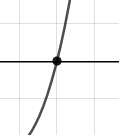
\includegraphics[width = 0.3\textwidth]{../Figures/polyZeroBehaviorCopyDA.png}
\end{multicols}\item None of the above.\end{enumerate}
\textbf{General Comment:} You will need to sketch the entire graph, then zoom in on the zero the question asks about.
}
\litem{
Describe the end behavior of the polynomial below.
\[ f(x) = -7(x + 2)^{3}(x - 2)^{6}(x - 3)^{5}(x + 3)^{7} \]The solution is the graph below, which is option A.
\begin{center}
    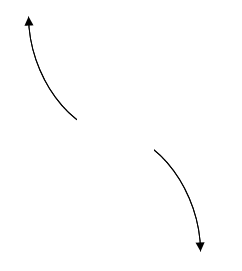
\includegraphics[width=0.3\textwidth]{../Figures/polyEndBehaviorCopyAA.png}
\end{center}\begin{enumerate}[label=\Alph*.]
\begin{multicols}{2}
\item 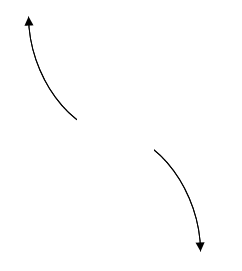
\includegraphics[width = 0.3\textwidth]{../Figures/polyEndBehaviorCopyAA.png}
\item 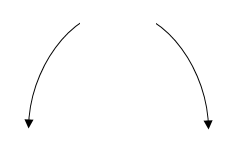
\includegraphics[width = 0.3\textwidth]{../Figures/polyEndBehaviorCopyBA.png}
\item 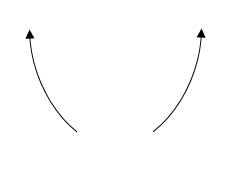
\includegraphics[width = 0.3\textwidth]{../Figures/polyEndBehaviorCopyCA.png}
\item 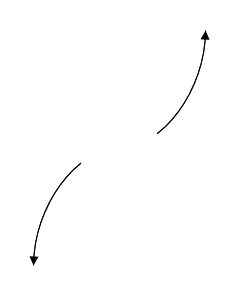
\includegraphics[width = 0.3\textwidth]{../Figures/polyEndBehaviorCopyDA.png}
\end{multicols}\item None of the above.\end{enumerate}
\textbf{General Comment:} Remember that end behavior is determined by the leading coefficient AND whether the \textbf{sum} of the multiplicities is positive or negative.
}
\litem{
Describe the end behavior of the polynomial below.
\[ f(x) = 9(x - 6)^{3}(x + 6)^{8}(x - 7)^{3}(x + 7)^{4} \]The solution is the graph below, which is option C.
\begin{center}
    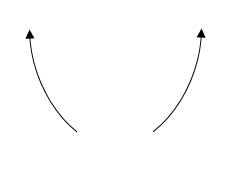
\includegraphics[width=0.3\textwidth]{../Figures/polyEndBehaviorCA.png}
\end{center}\begin{enumerate}[label=\Alph*.]
\begin{multicols}{2}
\item 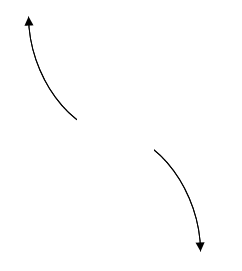
\includegraphics[width = 0.3\textwidth]{../Figures/polyEndBehaviorAA.png}
\item 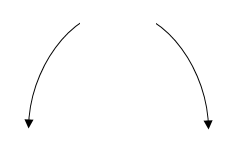
\includegraphics[width = 0.3\textwidth]{../Figures/polyEndBehaviorBA.png}
\item 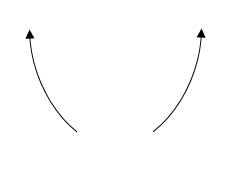
\includegraphics[width = 0.3\textwidth]{../Figures/polyEndBehaviorCA.png}
\item 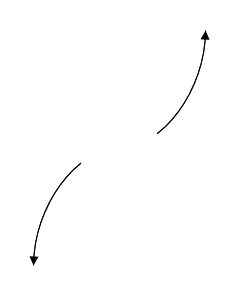
\includegraphics[width = 0.3\textwidth]{../Figures/polyEndBehaviorDA.png}
\end{multicols}\item None of the above.\end{enumerate}
\textbf{General Comment:} Remember that end behavior is determined by the leading coefficient AND whether the \textbf{sum} of the multiplicities is positive or negative.
}
\litem{
Which of the following equations \textit{could} be of the graph presented below?

\begin{center}
    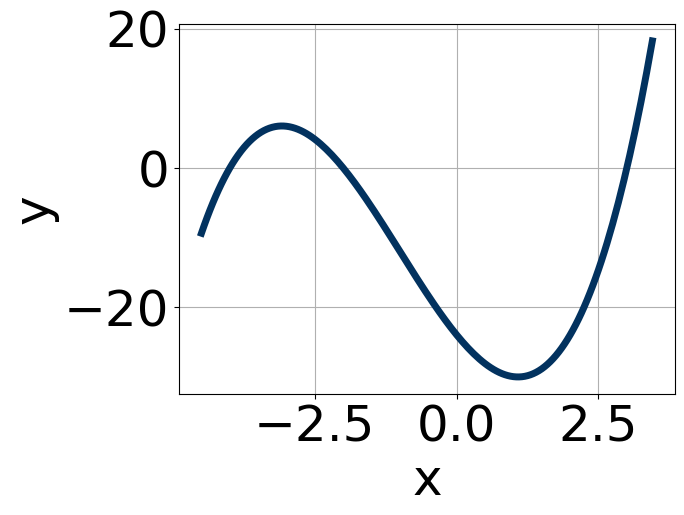
\includegraphics[width=0.5\textwidth]{../Figures/polyGraphToFunctionCopyA.png}
\end{center}


The solution is \( 20(x + 4)^{10} (x + 2)^{8} (x - 1)^{8} \), which is option E.\begin{enumerate}[label=\Alph*.]
\item \( -8(x + 4)^{10} (x + 2)^{10} (x - 1)^{8} \)

This corresponds to the leading coefficient being the opposite value than it should be.
\item \( -15(x + 4)^{4} (x + 2)^{10} (x - 1)^{7} \)

The factor $(x - 1)$ should have an even power and the leading coefficient should be the opposite sign.
\item \( 16(x + 4)^{10} (x + 2)^{8} (x - 1)^{9} \)

The factor $(x - 1)$ should have an even power.
\item \( 3(x + 4)^{4} (x + 2)^{5} (x - 1)^{7} \)

The factors $(x + 2)$ and $(x - 1)$ should both have even powers.
\item \( 20(x + 4)^{10} (x + 2)^{8} (x - 1)^{8} \)

* This is the correct option.
\end{enumerate}

\textbf{General Comment:} General Comments: Draw the x-axis to determine which zeros are touching (and so have even multiplicity) or cross (and have odd multiplicity).
}
\litem{
Construct the lowest-degree polynomial given the zeros below. Then, choose the intervals that contain the coefficients of the polynomial in the form $x^3+bx^2+cx+d$.
\[ 2 - 4 i \text{ and } -3 \]The solution is \( x^{3} -1 x^{2} +8 x + 60 \), which is option B.\begin{enumerate}[label=\Alph*.]
\item \( b \in [-0.9, 1.3], c \in [7.04, 8.22], \text{ and } d \in [-63, -58] \)

$x^{3} + x^{2} +8 x -60$, which corresponds to multiplying out $(x-(2 - 4 i))(x-(2 + 4 i))(x -3)$.
\item \( b \in [-1.3, 0.3], c \in [7.04, 8.22], \text{ and } d \in [58, 61] \)

* $x^{3} -1 x^{2} +8 x + 60$, which is the correct option.
\item \( b \in [-0.9, 1.3], c \in [0.36, 1.21], \text{ and } d \in [-9, -1] \)

$x^{3} + x^{2} +x -6$, which corresponds to multiplying out $(x -2)(x + 3)$.
\item \( b \in [-0.9, 1.3], c \in [6.7, 7.73], \text{ and } d \in [9, 17] \)

$x^{3} + x^{2} +7 x + 12$, which corresponds to multiplying out $(x + 4)(x + 3)$.
\item \( \text{None of the above.} \)

This corresponds to making an unanticipated error or not understanding how to use nonreal complex numbers to create the lowest-degree polynomial. If you chose this and are not sure what you did wrong, please contact the coordinator for help.
\end{enumerate}

\textbf{General Comment:} Remember that the conjugate of $a+bi$ is $a-bi$. Since these zeros always come in pairs, we need to multiply out $(x-(2 - 4 i))(x-(2 + 4 i))(x-(-3))$.
}
\end{enumerate}

\end{document}